% ==========================================================================
\section{Operating System (OS)}
% ==========================================================================
dzOS (or DZOS) is a single-user single-task ROM-based operating system (OS)
for the 8-bit homebrew computer dastaZ80. It is heavily influenced by ideas
and paradigms coming from Digital Research, Inc. CP/M, so some concepts may
sound familiar to those who had used this operating system.

The user communicates with the OS via a keyboard and a screen connected
directly to the computer.

The main job of dzOS is to allow the user to run programs, one at a time and
communicate with the different peripherals (or devices, as referred in this
manual). The user types in a command and the operating system checks what to
do with the command received, to execute a set of instructions.

Other tasks of dzOS are: handling disk files via its file system (DZFS),
getting user input from the keyboard, writing messages on the screen and
receiving/sending data through the serial port.

dzOS consists of three parts:
\begin{itemize}
    \item The \textbf{BIOS}, that provides functions for controlling the
    hardware.
    \item The \textbf{Kernel}, which provides general functions for
    everything that is not hardware dependent.
    \item The Command-Line Interface (\textbf{CLI}), that provides commands
    for the user to talk to the Kernel and the BIOS.
\end{itemize}

The Kernel and the CLI are hardware independent and will work on other Z80
based computers. Therefore, by adapting the BIOS code, dzOS can easily be
ported to other Z80 systems.

    % ==========================================================================
    \subsection{dastaZ80 File System (DZFS)}
    % ==========================================================================
    A file system manages access to the data stored in a storage medium, a
    MicroSD card or a Floppy Disk in the case of dastaZ80, and allows the OS to
    load and save data in the device (from now on, referred as \textbf{DISK}).

    DZFS is my first time designing a file system and for this reason I kept it
    very simple.

    It uses \textit{Logical Block Addressing} (LBA) for accessing the data on the
    \textbf{DISK}, and an allocation table called \textit{Block Allocation
    Table} (or \textit{BAT} for short) based in blocks of sectors.

    A \textbf{DISK} in DZFS can be a maximum of 33,521,152 bytes (33 MB). The
    reason for this specific maximum is explained later in this section. The
    Z80 is a 16-bit addressing CPU, and hence it can only access a maximum of
    65,536 addresses. Therefore, it would be impossible for the CPU to access
    bytes with a higher address. To solve this, the data in the \textbf{DISK} is
    virtually grouped into Sectors. Each Sector is a group of 512 bytes.
    Therefore, we have 65,472 Sectors (33,521,664 / 512) per disk, which is
    addressable by the CPU.

    For this reason, the BAT is really not allocating Blocks but Sectors, it
    should instead have been more correctly named \textit{Sector Allocation
    Table}.

    As the free RAM of dastaZ80 is about 48 KB, it makes no sense to have files
    bigger than that, as it would not fit into \textbf{MEMORY}. Therefore, I
    have decided that each Block can store only a single file.

    The file index is kept in an allocation table that occupies an entire Block
    (32,768 bytes) and each entry in the table is 32 bytes long. Therefore, the
    \textit{BAT} can allocate a maximum of 1,024 files (32,768 / 32).

    Because there is a maximum of 1,024 files, and each file can be a maximum
    of 32,768 bytes, the maximum amount of bytes that can be stored in a
    \textbf{DISK} is 33,554,432 bytes (32,768 x 1,024). The first 512 bytes
    are used by the \textit{Superblock} (to store \textbf{DISK} geometry and
    other details), and the BAT uses 32,768 bytes in itself. Therefore, there is
    a maximum space left for storing files of 33,521,152 bytes.

    Each entry in the \textit{BAT} holds information for each file in the disk;
    filename, attributes, time/date created, time/date last modified, file size,
    load address.

        % ==========================================================================
        \subsubsection{File Attributes}
        % ==========================================================================
        \label{subsub:fileattr}

        Files can have any of the following attributes:

        \begin{itemize}
            \item \textbf{Read Only} (R): it cannot be overwritten, renamed or
            deleted.
            \item \textbf{Hidden} (H): it does not show up in the results
            produced by the command \hyperref[cmd:cat]{cat}.
            \item \textbf{System} (S): this is a file used by DZOS and it MUST
            not be altered.
            \item \textbf{Executable} (E): this is an executable file and can be
            run directly with the command \hyperref[cmd:run]{run}.
        \end{itemize}

        % ==========================================================================
        \subsubsection{File Types}
        % ==========================================================================
        \label{subsub:filetypes}

        \begin{itemize}
            \item \textbf{USR}: User defined.
            \item \textbf{EXE}: Executable binary. Meant to be run with the 
                \hyperref[cmd:run]{run} command.
            \item \textbf{BIN}: Binary (non-executable) data. Meant to be loaded
            \   into \textbf{MEMORY} with the \hyperref[cmd:load]{load} command.
            \item \textbf{BAS}: BASIC code. Meant to be laoded with
                \hyperref[sub:msbasic]{MS BASIC}.
            \item \textbf{TXT}: Plain ASCII Text file.
            \item \textbf{FN6}: Font (6×8) for Text Mode. Meant to be loaded
                with the \hyperref[sub:loadfont]{loadfont} tool.
            \item \textbf{FN8}: Font (8×8) for Graphics Modes. Meant to be
                loaded with the \hyperref[sub:loadfont]{loadfont} tool.
            \item \textbf{SC1}: Screen 1 (Graphics I Mode) Picture. Meant to be
                loaded with the \hyperref[sub:loadscr]{loadscr} tool.
            \item \textbf{SC2}: Screen 2 (Graphics II Mode) Picture. Meant to be
                loaded with the \hyperref[sub:loadscr]{loadscr} tool.
            \item \textbf{SC3}: Screen 3 (Multicolour Mode) Picture. Meant to be
                loaded with the \hyperref[sub:loadscr]{loadscr} tool.
        \end{itemize}

        % ==========================================================================
        \subsubsection{DZFS limitations}
        % ==========================================================================
        The current version of the DZFS implementation (DZFSV1) have the following
        limitations:

        \begin{itemize}
            \item No support for directories. All files are presented at the same
            level.
            \item Filenames:
            \begin{itemize}
                \item Are case sensitive.
                \item Can be maximum 14 characters long.
                \item Can only contain alphabetical (A to Z) and numerical (0 to 9)
                    letters.
                \item Cannot start with a number.
                \item No support for extensions. But it uses attribute
                    \hyperref[subsub:filetypes]{File Type} instead.
            \end{itemize}
            \item Maximum size for a file is 32,768 bytes.
        \end{itemize}
        
    % ==========================================================================
    \subsection{The Command Prompt}
    % ==========================================================================
    When you switch ON the computer, you will hear a low tone (beep).

    The \textbf{Low Resolution Display} will display a welcome text and the 
    \textbf{High Resolution Display} will show some information:

    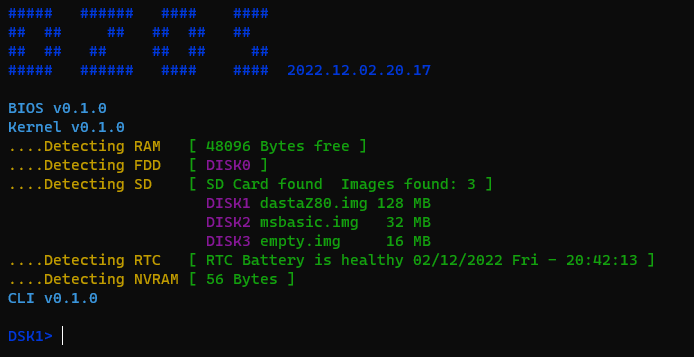
\includegraphics[scale=0.6]{images/dzOS.png}

    This information tells you about the release version of DZOS (2022.07.19.13
    in the screenshot). The BIOS, Kernel and CLI versions, and the detection of
    the different devices used by the computer. It also tells about whichs 
    \textbf{DISK}s are available.

    After that information,you will see the \textit{command prompt}. It starts
    with the letters \textit{DSK} (short for DISK) and a number, followed by the
    symbol $>$

    The number indicates which \textbf{DISK} is currently used for \textbf{DISK}
    operations.

    In other words, if you see \textit{DSK0}, it means that the Floppy Disk Drive
    (\textbf{FDD}) is selected. Entering commands like \textit{cat},
    \textit{diskinfo}, \textit{load}, etc., will instruct the computer to do it
    on the \textbf{FDD}.